\chapter{Gráficos e diagramas}

\chapterquote{``Citação.''}{Autor}

% --------

\section{Introdução ao \texttt{TikZ} e \texttt{pgfplots}}

Use o pacote \verb|geometry| para ajustar margens, cabeçalhos e rodapés:

\begin{itemize}
    \item \verb|TikZ|: Pacote para criação de gráficos vetoriais, diagramas e ilustrações complexas diretamente no LaTeX.
    \item \verb|pgfplots|: Extensão do TikZ para plotagem de dados e funções matemáticas.
\end{itemize}   

\begin{lstlisting}[language=tex, caption=Carregue os pacotes essenciais]
    \usepackage{tikz}
    \usepackage{pgfplots}
    \pgfplotsset{compat=1.18} % Define a versão para compatibilidade
    \usetikzlibrary{shapes, arrows.meta, positioning} % Bibliotecas úteis
\end{lstlisting} 

\section{Exemplos}

\subsection{Linhas e pontos}

\begin{lstlisting}[language=tex, caption={Linhas e pontos}]
    \begin{center}
        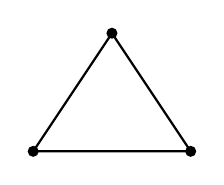
\begin{tikzpicture}
            \draw[thick] (0,0) -- (2,0) -- (1,1.5) -- cycle;
            \foreach \point in {(0,0), (2,0), (1,1.5)}
            \fill \point circle (2pt);
        \end{tikzpicture}
    \end{center}
\end{lstlisting} 


\begin{center}
    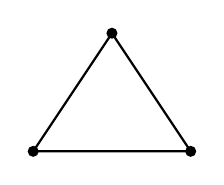
\begin{tikzpicture}
        \draw[thick] (0,0) -- (2,0) -- (1,1.5) -- cycle;
        \foreach \point in {(0,0), (2,0), (1,1.5)}
        \fill \point circle (2pt);
    \end{tikzpicture}
\end{center}

\begin{itemize}
    \item Espessuras: \verb|ultra thin|, \verb|very thin|, \verb|thin|, \verb|semithick|, \verb|thick|, \verb|very thick|, \verb|ultra thick|
    \item Espessura específica:\\\verb|\draw[line width=1.5pt] (0,0) -- (2,0) -- (1,1.5) -- cycle;|
\end{itemize}

\subsection{Retângulo e círculo}

\begin{lstlisting}[language=tex, caption=Retângulo e círculo]
    \begin{center}
        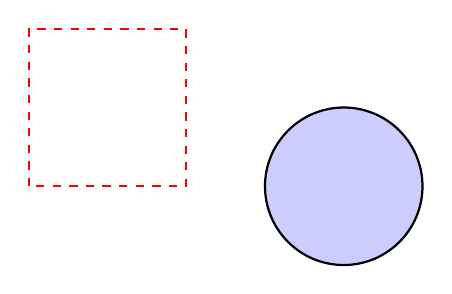
\begin{tikzpicture}
            \draw[thick, dashed, red] (-1,0) rectangle (1,2);
            \draw[thick, fill=blue!20] (3,0) circle (1cm);
        \end{tikzpicture}
    \end{center}
\end{lstlisting} 

\begin{center}
    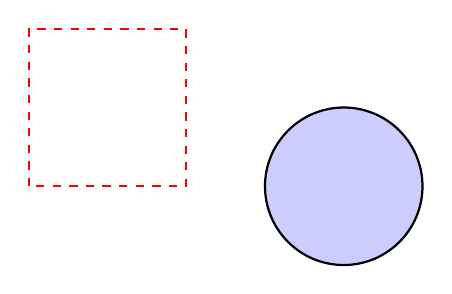
\begin{tikzpicture}
        \draw[thick, dashed, red] (-1,0) rectangle (1,2);
        \draw[thick, fill=blue!20] (3,0) circle (1cm);
    \end{tikzpicture}
\end{center}

\subsection{Diagramas de fluxo}

\begin{lstlisting}[language=tex, caption=Diagramas de fluxo]
    \begin{center}
        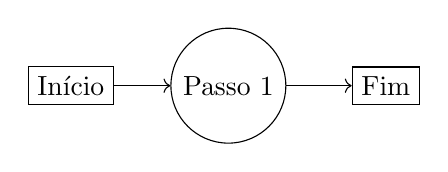
\begin{tikzpicture}
            \node (start) at (-2,0) [draw, rectangle] {Início};
            \node (step1) at (0,0) [draw, circle] {Passo 1};
            \node (end) at (2,0) [draw, rectangle] {Fim};
        
            \draw[->] (start) -- (step1);
            \draw[->] (step1) -- (end);
        \end{tikzpicture}
    \end{center}
\end{lstlisting} 

\begin{center}
    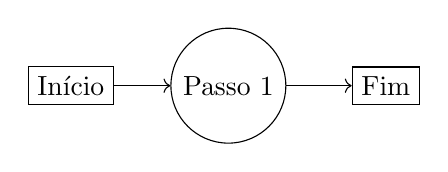
\begin{tikzpicture}
        \node (start) at (-2,0) [draw, rectangle] {Início};
        \node (step1) at (0,0) [draw, circle] {Passo 1};
        \node (end) at (2,0) [draw, rectangle] {Fim};
    
        \draw[->] (start) -- (step1);
        \draw[->] (step1) -- (end);
    \end{tikzpicture}
\end{center}

\subsection{Gráfico de Função Senoidal}

\begin{lstlisting}[language=tex, caption=Gráfico de Função Senoidal]
    \begin{center}
        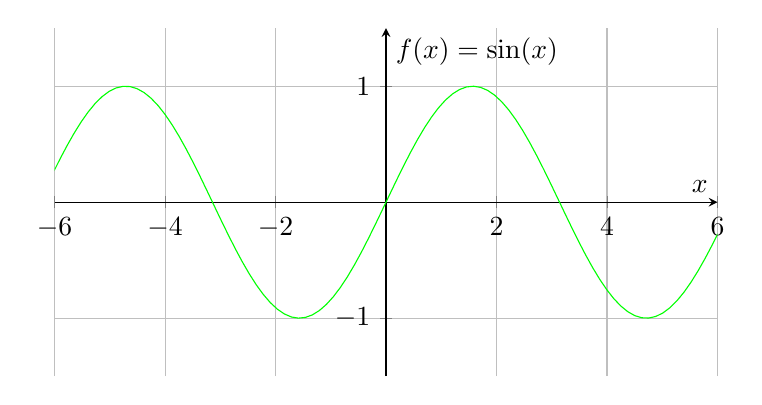
\begin{tikzpicture}
            \begin{axis}[
                axis lines = middle,
                xlabel = \(x\),
                ylabel = {\(f(x) = \sin(x)\)},
                xmin = -6, xmax = 6,
                ymin = -1.5, ymax = 1.5,
                grid = major,
                width=10cm,
                height=6cm
            ]
            \addplot[domain=-2*pi:2*pi, samples=100, color=green] {sin(deg(x))};
            \end{axis}
        \end{tikzpicture}
    \end{center}
\end{lstlisting} 

\begin{center}
    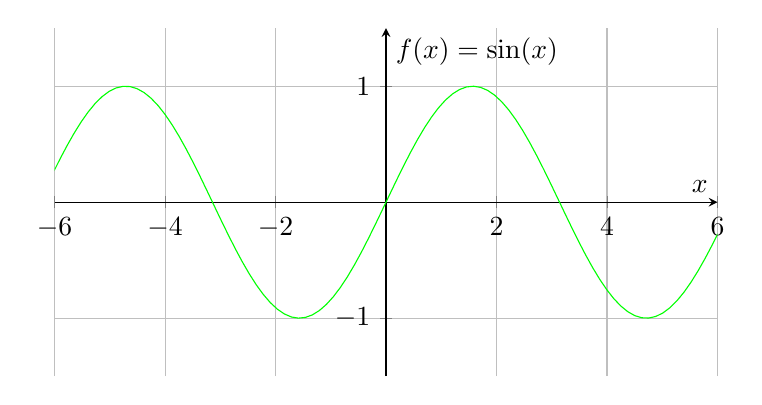
\begin{tikzpicture}
        \begin{axis}[
            axis lines = middle,
            xlabel = \(x\),
            ylabel = {\(f(x) = \sin(x)\)},
            xmin = -6, xmax = 6,
            ymin = -1.5, ymax = 1.5,
            grid = major,
            width=10cm,
            height=6cm
        ]
        \addplot[domain=-2*pi:2*pi, samples=100, color=green] {sin(deg(x))};
        \end{axis}
    \end{tikzpicture}
\end{center}

\subsection{Gráfico de barras e dados}

\begin{lstlisting}[language=tex, caption=Gráfico de barras]
    \begin{center}
        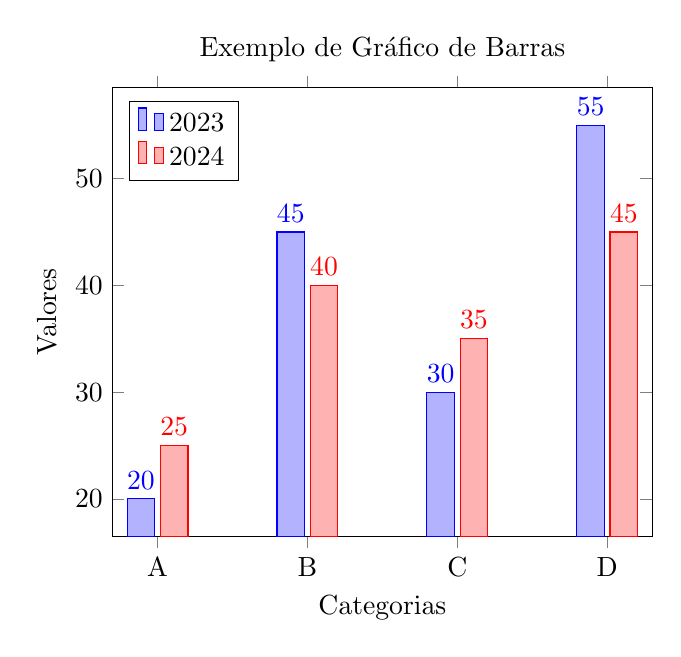
\begin{tikzpicture}
            \begin{axis}[
                ybar,
                symbolic x coords={A,B,C,D},
                xtick=data,
                nodes near coords,
                xlabel=Categorias,
                ylabel=Valores,
                title={Exemplo de Gráfico de Barras},
                legend pos=north west
            ]
            \addplot coordinates {(A,20) (B,45) (C,30) (D,55)};
            \addplot coordinates {(A,25) (B,40) (C,35) (D,45)};
            \legend{2023, 2024}
            \end{axis}
        \end{tikzpicture}
    \end{center}
\end{lstlisting} 

\begin{center}
    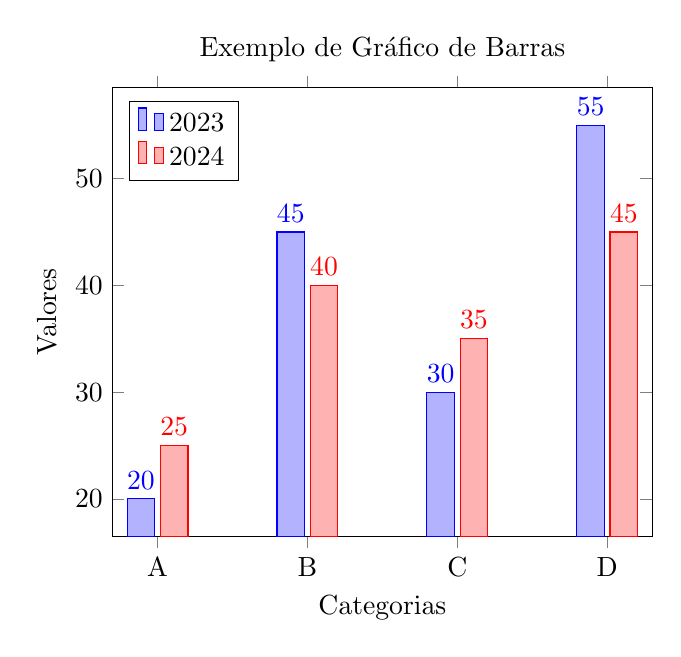
\begin{tikzpicture}
        \begin{axis}[
            ybar,
            symbolic x coords={A,B,C,D},
            xtick=data,
            nodes near coords,
            xlabel=Categorias,
            ylabel=Valores,
            title={Exemplo de Gráfico de Barras},
            legend pos=north west
        ]
        \addplot coordinates {(A,20) (B,45) (C,30) (D,55)};
        \addplot coordinates {(A,25) (B,40) (C,35) (D,45)};
        \legend{2023, 2024}
        \end{axis}
    \end{tikzpicture}
\end{center}

\subsection{Diagrama de Venn}

\begin{lstlisting}[language=tex, caption=Diagrama de Venn]
    \begin{center}
        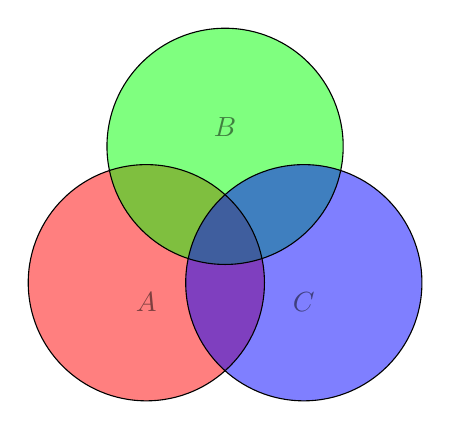
\begin{tikzpicture}
            \centering
            \begin{scope}[shift={(3cm,-5cm)}, fill opacity=0.5]
                \fill[red] \firstcircle;
                \fill[green] \secondcircle;
                \fill[blue] \thirdcircle;
                \draw \firstcircle node[below] {$A$};
                \draw \secondcircle node [above] {$B$};
                \draw \thirdcircle node [below] {$C$};
            \end{scope}
        \end{tikzpicture}
    \end{center}
\end{lstlisting} 

\def\firstcircle{(0,0) circle (1.5cm)}
\def\secondcircle{(60:2cm) circle (1.5cm)}
\def\thirdcircle{(0:2cm) circle (1.5cm)}

\begin{center}
    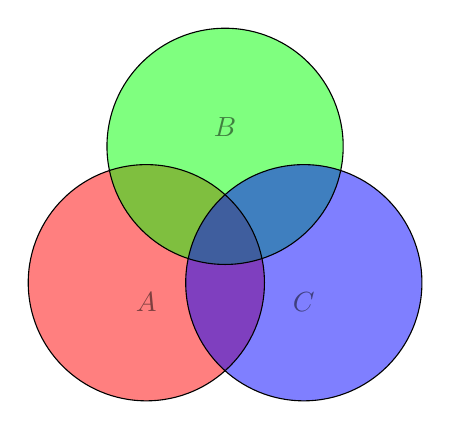
\begin{tikzpicture}
        \centering
        \begin{scope}[shift={(3cm,-5cm)}, fill opacity=0.5]
            \fill[red] \firstcircle;
            \fill[green] \secondcircle;
            \fill[blue] \thirdcircle;
            \draw \firstcircle node[below] {$A$};
            \draw \secondcircle node [above] {$B$};
            \draw \thirdcircle node [below] {$C$};
        \end{scope}
    \end{tikzpicture}
\end{center}

\subsection{Superfície 3D (função matemática)}

\begin{lstlisting}[language=tex, caption=Superfície 3D de função matemática]
    \begin{center}
        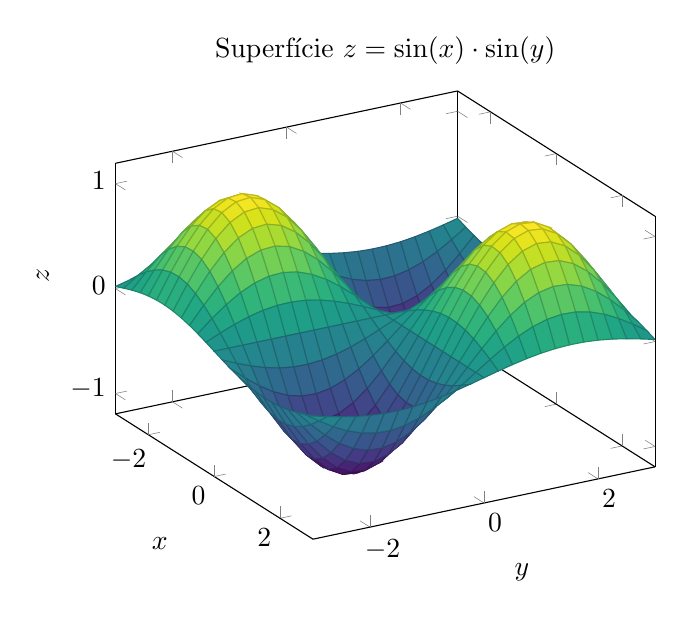
\begin{tikzpicture}
            \begin{axis}[
                view={60}{30}, % Ângulo de visualização (azimute, elevação)
                xlabel = \(x\),
                ylabel = \(y\),
                zlabel = \(z\),
                title = {Superfície \(z = \sin(x) \cdot \sin(y)\)},
                colormap/viridis, % Esquema de cores
            ]
            \addplot3[
                surf,
                domain = -3:3,
                domain y = -3:3,
                samples = 25,
            ] 
                {sin(deg(x)) * sin(deg(y))};
            \end{axis}
        \end{tikzpicture}
    \end{center}
\end{lstlisting} 

\begin{center}
    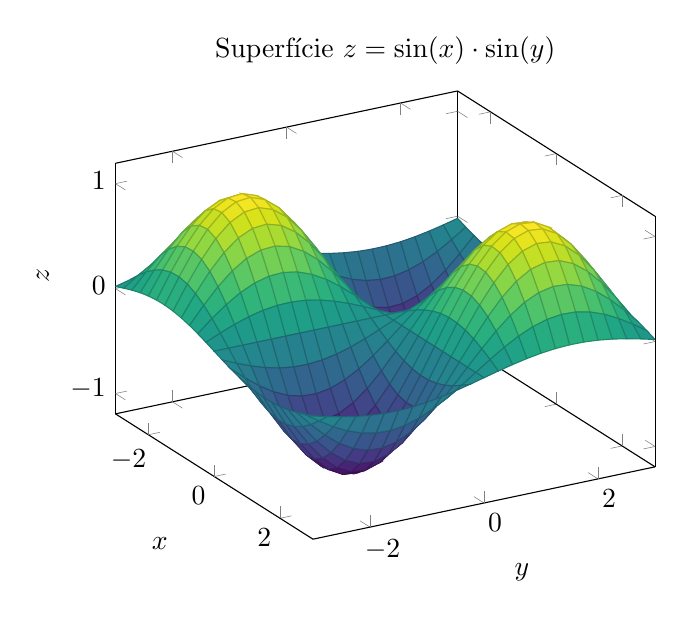
\begin{tikzpicture}
        \begin{axis}[
            view={60}{30}, % Ângulo de visualização (azimute, elevação)
            xlabel = \(x\),
            ylabel = \(y\),
            zlabel = \(z\),
            title = {Superfície \(z = \sin(x) \cdot \sin(y)\)},
            colormap/viridis, % Esquema de cores
        ]
        \addplot3[
            surf,
            domain = -3:3,
            domain y = -3:3,
            samples = 25,
        ] 
            {sin(deg(x)) * sin(deg(y))};
        \end{axis}
    \end{tikzpicture}
\end{center}

\subsection{Gráfico de Dispersão 3D}

\begin{lstlisting}[language=tex, caption=Gráfico de Dispersão 3D]
    \begin{center}
        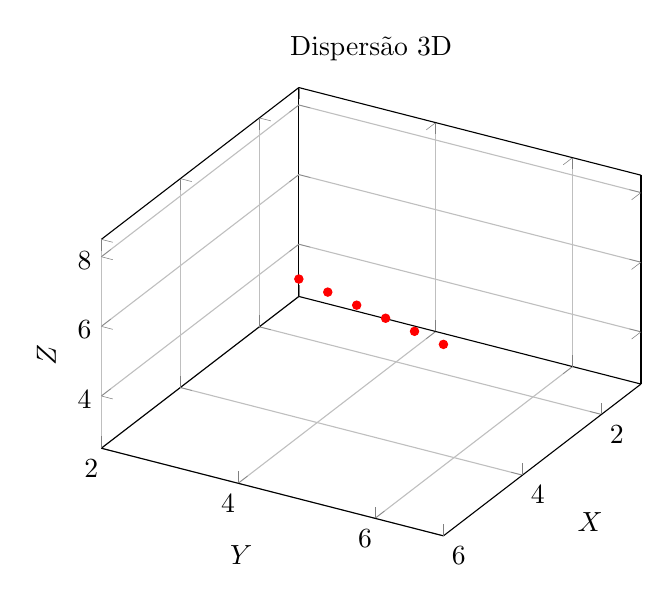
\begin{tikzpicture}
            \begin{axis}[
                view={120}{40},
                xlabel = \(X\),
                ylabel = \(Y\),
                zlabel = \(Z\),
                title = {Dispersão 3D},
                grid = major,
            ]
            \addplot3[
                only marks,
                mark = *,
                mark size = 1.5pt,
                color = red,
            ] coordinates {
                (1,2,3) (2,3,4) (3,4,5)
                (4,5,6) (5,6,7) (6,7,8)
            };
            \end{axis}
        \end{tikzpicture}
    \end{center}
\end{lstlisting} 

\begin{center}
    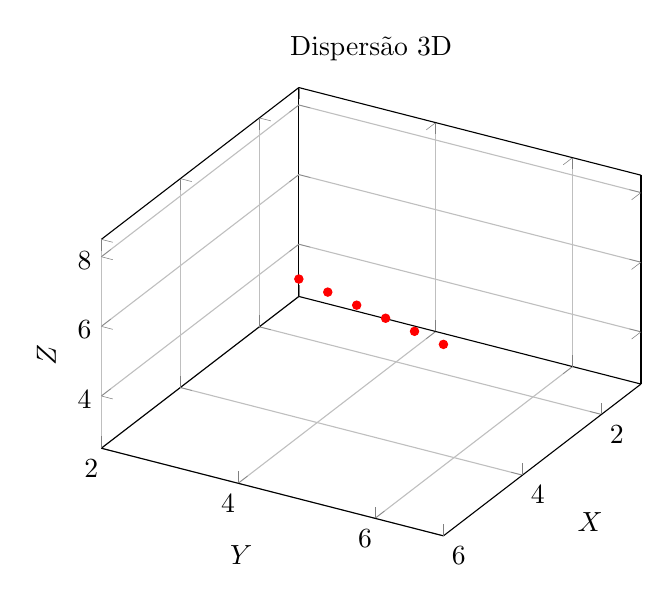
\begin{tikzpicture}
        \begin{axis}[
            view={120}{40},
            xlabel = \(X\),
            ylabel = \(Y\),
            zlabel = \(Z\),
            title = {Dispersão 3D},
            grid = major,
        ]
        \addplot3[
            only marks,
            mark = *,
            mark size = 1.5pt,
            color = red,
        ] coordinates {
            (1,2,3) (2,3,4) (3,4,5)
            (4,5,6) (5,6,7) (6,7,8)
        };
        \end{axis}
    \end{tikzpicture}
\end{center}

\subsection{Gráfico Paramétrico (hélice)}

\begin{lstlisting}[language=tex, caption=Gráfico Paramétrico (hélice)]
    \begin{center}
        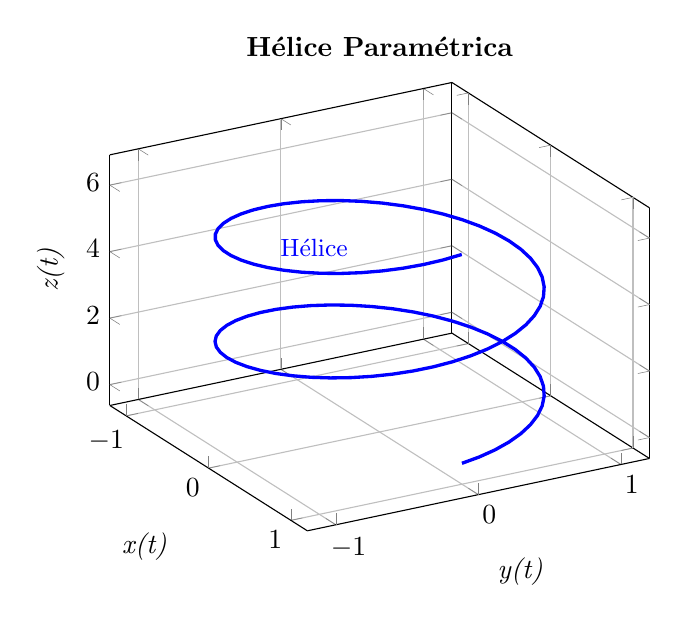
\begin{tikzpicture}
            \begin{axis}[
                view={60}{30}, % Alterado para uma visão mais tridimensional
                xlabel = {\textit{x(t)}},
                ylabel = {\textit{y(t)}},
                zlabel = {\textit{z(t)}},
                title = {\textbf{Hélice Paramétrica}},
                grid = major, % Adiciona grade para melhor visualização
                xtick = {-1, 0, 1},
                ytick = {-1, 0, 1},
                ztick = {0, 2, 4, 6}, % Ajustando os ticks do eixo z
                enlargelimits = 0.1,
                legend pos=north east, % Posição da legenda
            ]
            \addplot3[
                domain = 0:4*pi,
                samples = 100,
                samples y = 0,
                color = blue,
                very thick, % Linha mais grossa para destaque
            ] 
                ({cos(deg(x))}, {sin(deg(x))}, {x/2}) 
                node[pos=0.9,anchor=south west] {\small Hélice};
            \end{axis}
        \end{tikzpicture}
\end{center}
\end{lstlisting} 

\begin{center}
    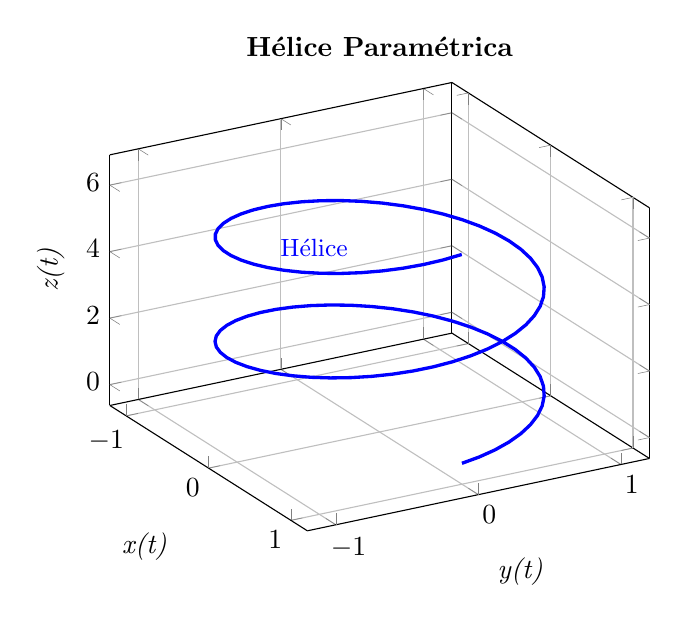
\begin{tikzpicture}
        \begin{axis}[
            view={60}{30}, % Alterado para uma visão mais tridimensional
            xlabel = {\textit{x(t)}},
            ylabel = {\textit{y(t)}},
            zlabel = {\textit{z(t)}},
            title = {\textbf{Hélice Paramétrica}},
            grid = major, % Adiciona grade para melhor visualização
            xtick = {-1, 0, 1},
            ytick = {-1, 0, 1},
            ztick = {0, 2, 4, 6}, % Ajustando os ticks do eixo z
            enlargelimits = 0.1,
            legend pos=north east, % Posição da legenda
        ]
        \addplot3[
            domain = 0:4*pi,
            samples = 100,
            samples y = 0,
            color = blue,
            very thick, % Linha mais grossa para destaque
        ] 
            ({cos(deg(x))}, {sin(deg(x))}, {x/2}) 
            node[pos=0.9,anchor=south west] {\small Hélice};
        \end{axis}
    \end{tikzpicture}
\end{center}

\subsection{Gráfico de contorno 3D}

\begin{lstlisting}[language=tex, caption=Gráfico de contorno 3D]
    \begin{center}
        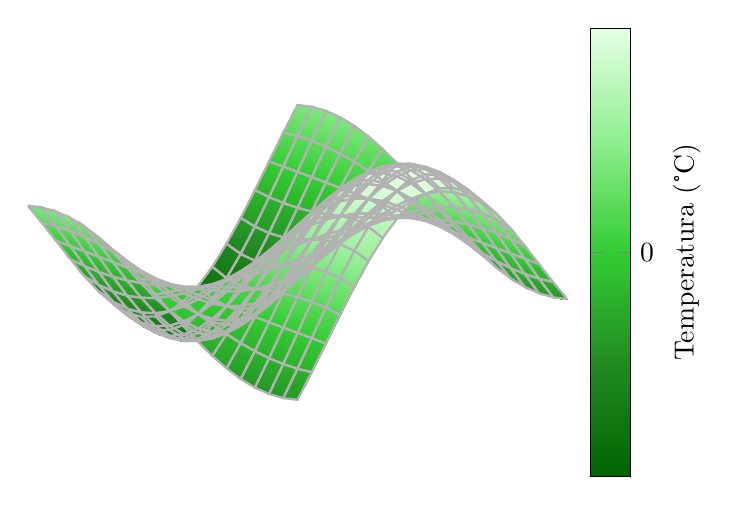
\begin{tikzpicture}
            \begin{axis}[
                view={45}{30}, % Ângulo ajustado para melhor visualização
                colormap={customgreen}{ % Paleta verde suave e equilibrada
                    rgb255(0cm)=(0,100,0)   % Verde escuro
                    rgb255(1cm)=(34,139,34) % Verde floresta
                    rgb255(2cm)=(50,205,50) % Verde lima
                    rgb255(3cm)=(144,238,144) % Verde claro
                    rgb255(4cm)=(230,255,230) % Verde quase branco
                },
                enlargelimits=false,
                hide axis, % Remove eixos para um visual mais clean
                colorbar, % Adiciona barra lateral de cores
                colorbar style={
                    ylabel={Temperatura (°C)}, % Rótulo da escala
                    ytick={-1,0,1,2,3,4}, % Marcas da barra de cores
                }
            ]
                % Superfície 3D ondulada com interpolação de cores
                \addplot3[
                    surf, % Superfície 3D
                    shader=interp, % Suaviza a transição de cores
                    domain=-2:2, y domain=-2:2, % Domínio dos eixos
                    samples=40, % Número de pontos para maior suavidade
                    samples y=40
                ]
                {sin(deg(x)) * cos(deg(y))}; % Função matemática ondulada
    
                % Adicionando a grid na superfície para um efeito visual aprimorado
                \addplot3[
                    mesh, % Plota uma malha (grid) na superfície
                    domain=-2:2, y domain=-2:2, 
                    samples=20, % Define quantos segmentos terá a malha
                    samples y=20,
                    thick, % Deixa as linhas da grid mais visíveis
                    black!30 % Define a cor da grid como cinza escuro (30% preto)
                ]
                {sin(deg(x)) * cos(deg(y))};
            \end{axis}
        \end{tikzpicture}
    \end{center}
\end{lstlisting} 

\begin{center}
    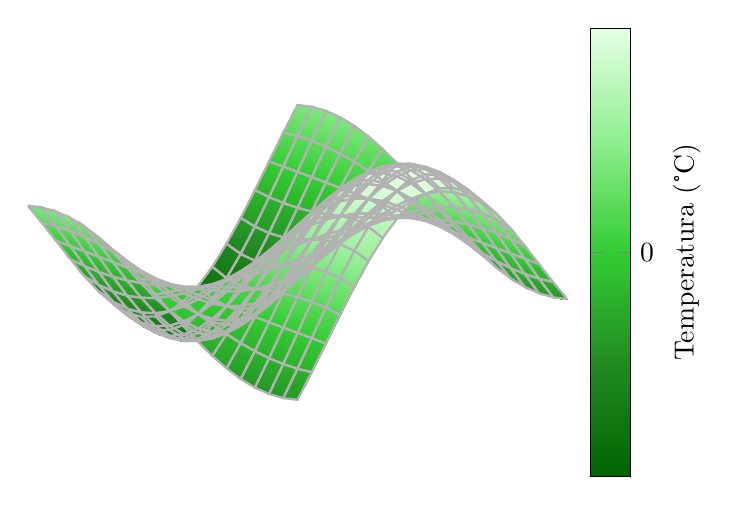
\begin{tikzpicture}
        \begin{axis}[
            view={45}{30}, % Ângulo ajustado para melhor visualização
            colormap={customgreen}{ % Paleta verde suave e equilibrada
                rgb255(0cm)=(0,100,0)   % Verde escuro
                rgb255(1cm)=(34,139,34) % Verde floresta
                rgb255(2cm)=(50,205,50) % Verde lima
                rgb255(3cm)=(144,238,144) % Verde claro
                rgb255(4cm)=(230,255,230) % Verde quase branco
            },
            enlargelimits=false,
            hide axis, % Remove eixos para um visual mais clean
            colorbar, % Adiciona barra lateral de cores
            colorbar style={
                ylabel={Temperatura (°C)}, % Rótulo da escala
                ytick={-1,0,1,2,3,4}, % Marcas da barra de cores
            }
        ]
            % Superfície 3D ondulada com interpolação de cores
            \addplot3[
                surf, % Superfície 3D
                shader=interp, % Suaviza a transição de cores
                domain=-2:2, y domain=-2:2, % Domínio dos eixos
                samples=40, % Número de pontos para maior suavidade
                samples y=40
            ]
            {sin(deg(x)) * cos(deg(y))}; % Função matemática ondulada

            % Adicionando a grid na superfície para um efeito visual aprimorado
            \addplot3[
                mesh, % Plota uma malha (grid) na superfície
                domain=-2:2, y domain=-2:2, 
                samples=20, % Define quantos segmentos terá a malha
                samples y=20,
                thick, % Deixa as linhas da grid mais visíveis
                black!30 % Define a cor da grid como cinza escuro (30% preto)
            ]
            {sin(deg(x)) * cos(deg(y))};
        \end{axis}
    \end{tikzpicture}
\end{center}

\section{Dicas práticas}

\begin{itemize}
    \item \href{https://tikz.dev/}{Manual do \texttt{TikZ}}.
    \item \href{https://pgfplots.sourceforge.net/}{Manual do \texttt{pgfplots}}.
    \item Templates: Explore modelos prontos em \href{https://texample.net/}{TeXample.net}.
\end{itemize}